\section{Architettura MongoDB}

MongoDB è un \textbf{sistema distribuito} basato su due principi fondamentali:

\begin{itemize}
	\item \textbf{Replicazione}: garantisce una maggiore resistenza in presenza di guasti. Consiste nella disseminazione di più copie identiche dello stesso dato su server diversi, aumentando l'\textbf{affidabilità} del sistema.
	
	\item \textbf{Sharding}: letteralmente \textit{frammentazione}, suddivide un dataset di grandi dimensioni in parti più piccole, garantendo la \textbf{scalabilità orizzontale}. Ogni shard può a sua volta essere replicato.
\end{itemize}

La \textbf{scalabilità orizzontale} consiste nell'aumentare la capacità del sistema aggiungendo nuovi nodi (macchine) alla rete, anziché potenziare le risorse di un singolo nodo (scalabilità verticale).

\subsection*{Replica Set}

Un \textbf{replica set} è una collezione di processi \texttt{mongod} che mantengono una copia dello stesso dataset. I vantaggi principali sono:

\begin{itemize}
	\item \textbf{Ridondanza e alta disponibilità}: aumenta la tolleranza ai guasti.
	\item \textbf{Manutenzione non invasiva}: permette di aggiornare hardware o software di un singolo nodo senza interrompere il servizio.
	\item \textbf{Miglioramento delle prestazioni} per le operazioni di lettura.
\end{itemize}

\subsection*{Funzionamento del Replica Set}

I dati contenuti nel nodo \textbf{Primary} vengono replicati nei nodi \textbf{Secondary}, che si coordinano e si mantengono sincronizzati attraverso un meccanismo di \textbf{heartbeat}: una sorta di battito cardiaco che permette ai nodi di monitorarsi reciprocamente.
\begin{figure}[H]
	\centering
	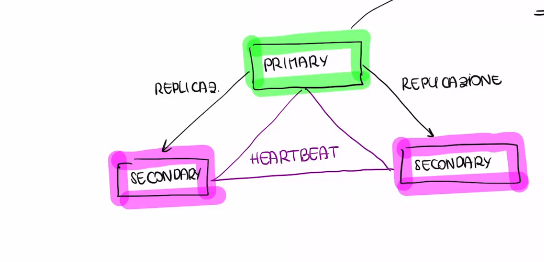
\includegraphics[width=0.7\linewidth]{iamge250}
	\caption{Schema di un Replica Set con nodo Primary e due nodi Secondary.}
	\label{fig:iamge250}
\end{figure}

In questo sistema distribuito, l'architettura è \textbf{fortemente centralizzata}:

\begin{itemize}
	\item Il nodo \textbf{Primary} gestisce tutte le operazioni di \textbf{scrittura}, mantenendo un log dei cambiamenti chiamato \textbf{oplog} (\textit{operations log}).
	\item All'interno di un replica set può esistere \textbf{un solo nodo Primary}.
	\item I nodi \textbf{Secondary} replicano le operazioni registrate nell'oplog, mantenendosi aggiornati rispetto al Primary.
\end{itemize}
\subsection*{Algoritmo di Elezione}

Tramite il meccanismo di \textbf{heartbeat}, se un nodo Secondary rileva che il nodo Primary non risponde, quest'ultimo viene dichiarato non disponibile e un nodo Secondary qualificato viene \textbf{eletto} nuovo Primary.

Questo meccanismo è detto \textbf{algoritmo di elezione} e segue il \textbf{protocollo di consenso Raft}.

\medskip
L'algoritmo di elezione viene attivato nei seguenti casi:

\begin{itemize}
	\item \textbf{Errore di comunicazione}: un nodo Secondary non riesce a comunicare con il Primary oltre un certo timeout (solitamente \textbf{10 secondi}) $\Rightarrow$ identificazione automatica della perdita del nodo Primary.
	\item \textbf{Inizializzazione} di un replica set: per stabilire quale nodo assume il ruolo di Primary.
	\item \textbf{Modifica} del replica set: quando si aggiunge o rimuove un nodo.
\end{itemize}

\subsubsection*{Come avviene l'elezione?}

L'algoritmo si basa su un \textbf{meccanismo di votazione} per determinare il nuovo nodo Primary, che non richiede più di \textbf{12 secondi}.

\begin{itemize}
	\item Il nodo Secondary con il \textbf{timestamp di scrittura più recente} ha la maggiore probabilità di vincere l'elezione.
	\item Per evitare elezioni continue, una volta conclusa l'elezione i nodi entrano in un \textbf{periodo di congelamento} durante il quale non possono avviare nuove elezioni (analogia: il termostato che, raggiunta la temperatura desiderata, non si spegne e riaccende immediatamente, ma attende un intervallo minimo).
\end{itemize}

\textbf{Nota importante}: fintanto che l'elezione non è conclusa, il replica set \textbf{non può eseguire operazioni di scrittura}, poiché queste competono esclusivamente al nodo Primary.

\subsection*{Oplog}

L'\textbf{oplog} (\textit{operations log}) è un log che contiene tutte le operazioni eseguite sui database gestiti da MongoDB.

\begin{itemize}
	\item Le operazioni di scrittura vengono prima eseguite sul \textbf{nodo Primary} e poi trascritte sui \textbf{nodi Secondary}.
	\item Esiste un oplog anche sui nodi Secondary.
	\item Le operazioni registrate nell'oplog sono \textbf{idempotenti}: applicarle più volte produce lo stesso risultato.
\end{itemize}

\subsection{Architettura del Replica Set}

Un replica set è formato di default da \textbf{tre membri}:
\begin{itemize}
	\item 1 nodo \textbf{Primary}
	\item 2 nodi \textbf{Secondary}
\end{itemize}

\subsection*{Best Practice}

\begin{itemize}
	\item I replica set devono contenere un \textbf{numero dispari di membri votanti}: i nodi Secondary devono essere in numero dispari, evitando situazioni di stallo dovute a parità di voti.
	
	\item Se non è possibile garantire la disparità, è necessaria la presenza di un \textbf{arbitro}: un nodo che partecipa alle votazioni ma non mantiene una copia dei dati e non può diventare nodo Primary.
	
	\item In architetture MongoDB reali esistono \textbf{membri nascosti} e \textbf{membri ritardati}, dedicati a task particolari come backup e reporting:
	\begin{itemize}
		\item Non possono diventare nodi Primary.
		\item Non sono direttamente accessibili dalle applicazioni client.
		\item I \textbf{nodi ritardati} replicano le operazioni del nodo Primary con un ritardo preimpostato, fungendo da fonte di \textbf{backup continuo}.
	\end{itemize}
	
	\item Almeno un nodo di ciascun replica set deve trovarsi in un \textbf{data center alternativo}.
\end{itemize}
\subsection{Replica Set: Gestione delle Scritture e Letture}

\subsubsection*{Write Concern}

È necessario un meccanismo per stabilire che i dati siano considerati scritti solo quando un certo numero di nodi secondari hanno replicato la scrittura. Questa proprietà è indicata come \textbf{write concern} e prevede tre parametri:

\begin{itemize}
	\item \texttt{w} = numero di nodi del replica set che devono aver confermato la scrittura prima che l'operazione sia considerata conclusa. I valori possibili sono:
	\begin{itemize}
		\item \texttt{0}: nessuna conferma richiesta
		\item \texttt{1}: solo il nodo Primary (default)
		\item \texttt{majority}: la maggioranza dei nodi
		\item \texttt{number}: un numero specifico di nodi
	\end{itemize}
	Aumentando \texttt{w} si riduce la latenza a favore della persistenza.
	\item \texttt{j} = richiede conferma che l'operazione di scrittura sia stata scritta su disco.
	\item \texttt{wtimeout} = limite in millisecondi oltre il quale, se l'operazione non è terminata, viene restituito un errore.
\end{itemize}

\subsubsection*{Read Preference}

Le operazioni di lettura vengono reindirizzate sul nodo Primary. Per aumentare le prestazioni è possibile distribuire le letture e bilanciare il carico attraverso le seguenti modalità:

\begin{itemize}
	\item \texttt{primary}: solo il nodo Primary (default)
	\item \texttt{primaryPreferred}: preferisce il Primary, usa un Secondary se non disponibile
	\item \texttt{secondary}: solo nodi Secondary
	\item \texttt{secondaryPreferred}: preferisce i Secondary, usa il Primary se non disponibile
	\item \texttt{nearest}: il nodo con la latenza più bassa
\end{itemize}

\subsubsection*{Read Concern}

Per garantire la consistenza dei dati letti, si utilizza il meccanismo di \textbf{read concern}:

\begin{itemize}
	\item \texttt{local}: restituisce il dato disponibile più recente nel nodo al momento della query, indipendentemente dallo stato di replicazione.
	\item \texttt{majority}: restituisce il dato confermato dalla maggioranza dei nodi del replica set $\Rightarrow$ alta consistenza.
	\item \texttt{linearizable}: restituisce il dato confermato da tutti i nodi $\Rightarrow$ massima consistenza.
	\item \texttt{snapshot}: restituisce i dati confermati dalla maggioranza dei nodi in un determinato momento.
\end{itemize}

\subsection{Sharding}

Lo \textbf{sharding} consiste nel suddividere un database in parti più piccole chiamate \textbf{shard}, dove ciascuno shard è un replica set che memorizza una porzione dei dati. Per gestire i dati partizionati su più shard sono necessari due componenti:

\begin{enumerate}
	\item \textbf{mongos}: router che distribuisce e reindirizza in modo efficiente le query tra i vari shard, consolida i risultati parziali e produce una risposta definitiva.
	\item \textbf{Config Server}: mantiene i metadati relativi allo sharding.
\end{enumerate}

\begin{figure}[H]
	\centering
	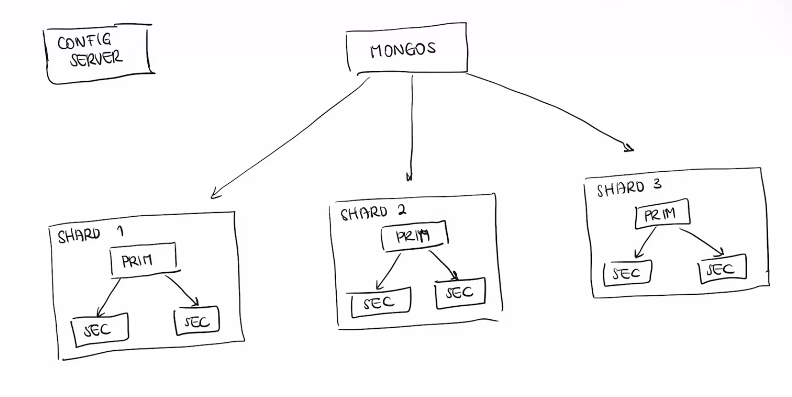
\includegraphics[width=0.7\linewidth]{image250}
	\caption{Architettura di sharding in MongoDB: mongos instrada le query verso i singoli shard, ciascuno composto da un replica set (Primary + Secondary).}
	\label{fig:image250}
\end{figure}


Il meccanismo di sharding offre \textbf{scalabilità orizzontale}.

\subsection*{Vantaggi dello Sharding}

\begin{itemize}
	\item Aumenta la velocità delle operazioni di lettura e scrittura.
	\item Aumenta la capacità di storage complessiva.
	\item \textbf{Zone sharding}: permette di sfruttare la località del dato.
\end{itemize}

\subsection*{Shard Key e Distribuzione dei Dati}

Lo sharding viene definito a livello di \textbf{collezione}, suddividendo i documenti in \textbf{chunk}. A ciascun shard è associata una \textbf{shard key}, dipendente da una o più proprietà dei documenti, utilizzata per distribuire i dati. A partire dalla versione 5.0 di MongoDB è supportato il \textbf{resharding}.

Le tecniche di distribuzione dei chunk sono:

\begin{itemize}
	\item \textbf{Ranged Sharding}: i dati vengono suddivisi in base a intervalli continui dei valori della shard key.
	\begin{itemize}
		\item Metodo di default.
		\item Ottimale per \textit{range query} sui valori della shard key.
		\item Il dominio dell'attributo chiave determina il numero di shard possibili.
		\item Valori molto frequenti possono generare chunk più numerosi e sbilanciati.
		\item Valori monotoni tendono a concentrare gli inserimenti sempre sullo stesso chunk.
	\end{itemize}
	\item \textbf{Hashed Sharding}: viene applicata una funzione hash al valore della shard key: valori simili producono hash diversi, garantendo una distribuzione più uniforme. Non efficiente per \textit{range query}.
\end{itemize}
\subsection*{Balancer}

Il \textbf{balancer} è un processo in background che assicura che la quantità di dati assegnata a ciascun shard sia la più bilanciata possibile. Quando la quantità di dati assegnati a uno shard raggiunge una soglia (\textit{threshold}), viene avviata una \textbf{redistribuzione} basata sul principio di località.

Casi particolari:

\begin{itemize}
	\item \textbf{Chunk indivisibile}: caratterizzato da un unico valore di chiave, non è bilanciabile. L'unica soluzione è il \textbf{resharding}.
	\item \textbf{Jumbo chunk}: chunk di dimensioni eccessive la cui suddivisione richiede un \textbf{intervento manuale}.
\end{itemize}

\subsection*{mongos}

Il server \textbf{mongos} amministra l'intero sistema, funge da \textbf{proxy server} e decide a quali shard devono essere instradate le query.

Le operazioni supportate includono: \texttt{find()}, \texttt{sort()}, \texttt{limit()}.

\subsection{Proprietà ACID in MongoDB}

\subsection*{A — Atomicità}

Tutte le operazioni che coinvolgono un \textbf{singolo documento} sono sempre atomiche, anche in caso di accesso a proprietà che sono documenti annidati o array.

Stima empirica: l'80--90\% delle applicazioni reali richiede query mono-documento. La dimensione massima di un documento in MongoDB è \textbf{16 MB}.

\subsection*{C — Consistenza}

\begin{itemize}
	\item \textbf{Strong consistency} (modello relazionale): ogni lettura futura restituisce sempre l'ultimo valore confermato $\Rightarrow$ penalizza le prestazioni.
	\item \textbf{Eventual consistency} (sistemi distribuiti): una volta che i dati sono stati aggiornati e propagati, tutte le letture future restituiranno eventualmente l'ultimo stato confermato $\Rightarrow$ alte prestazioni.
\end{itemize}

MongoDB adotta un \textbf{modello ibrido} che bilancia il numero di operazioni concorrenti e il livello di consistenza.

\subsection*{I — Isolamento}

Il livello di isolamento è controllato tramite \textbf{write concern} e \textbf{read concern}:

\begin{itemize}
	\item \texttt{local}: non garantisce che tutte le transazioni vedano lo stesso dato.
	\item \texttt{majority} / \texttt{snapshot}: tutte le transazioni vedono lo stesso risultato.
\end{itemize}

Se il write concern è impostato a \texttt{majority}, si garantisce che la scrittura sia propagata ad almeno la maggioranza dei nodi.

\subsection*{P — Persistenza}

MongoDB utilizza la stessa tecnica di PostgreSQL: il \textbf{Write-Ahead Log (WAL)}.